%===============================================================================
%===============================================================================
%
\clearpage
%
\subsection{Example-0201-u \texttt{[PLAUSIBLE]}}
%
Example uses generated or user-defined regular meshes in CHeart mesh format
and solves a static problem, i.e., applies the boundary conditions in one step.\\[3ex]

Issues: 2D, iterative solver, analytical Jacobian
%
%===============================================================================
%
\subsubsection{Mathematical model - 2D}
%
We solve the following scalar equation,
%
\begin{align}
    ...
\end{align}
%
with boundary conditions
%
\begin{align}
    ...
\end{align}
%
No material parameters to specify.
%
%===============================================================================
%
\subsubsection{Mathematical model - 3D}
%
We solve the following scalar equation,
%
\begin{align}
    ...
\end{align}
%
with boundary conditions
%
\begin{align}
    ...
\end{align}
%
No material parameters to specify.
%
%===============================================================================
%
\subsubsection{Computational model}
%
\begin{itemize}
    \item{Commandline arguments are:}
        \subitem{...}
        \subitem{}% quadratic simplex
    \item{Note: Binary uses command line arguments to search for the relevant mesh files.}
\end{itemize}
%
%===============================================================================
%
\subsubsection{Result summary}
%
We use iron reference results that were compared against an analytical solution.
%
\verbatiminput{examples/example-0201-u/results/results.summary}
\verbatiminput{examples/example-0201-u/results/failed.tests}
%
\begin{figure}[h!]
    \centering
%    \includegraphics[width=0.9\columnwidth]{examples/example-0201-u/doc/figures/iron_reference_2D.eps} 
    \caption{2D results, iron reference w/ command line arguments [...].}
    \label{example-0201-u-iron-2D-reference-fig}
\end{figure}
%
\begin{figure}[h!]
    \centering 
%    \includegraphics[width=0.9\columnwidth]{examples/example-0201-u/doc/figures/current_run_l2x1x0_n8x4x0_i1_s0.eps} 
    \caption{2D results, current run w/ command line arguments [...].}
    \label{example-0201-u-current-run-2D-fig}
\end{figure}
%
\begin{figure}[h!]
    \centering 
    \includegraphics[width=0.9\columnwidth]{examples/example-0201-u/doc/figures/iron_reference_3D.eps} 
    \caption{3D results, iron reference w/ command line arguments [...].}
    \label{example-0201-u-iron-3D-reference-fig}
\end{figure}
%
\begin{figure}[h!]
    \centering 
%    \includegraphics[width=0.9\columnwidth]{examples/example-0201-u/doc/figures/current_run_l2x1x1_n8x4x4_i1_s0.eps} 
    \caption{3D results, current run w/ command line arguments [...].}
    \label{example-0201-u-current-run-3D-fig}
\end{figure}
%
%===============================================================================
%===============================================================================
